%%=============================================================================
%% Methodologie
%%=============================================================================

\chapter{\IfLanguageName{dutch}{Methodologie}{Methodology}}
\label{ch:methodologie}

%% TODO: Hoe ben je te werk gegaan? Verdeel je onderzoek in grote fasen, en
%% licht in elke fase toe welke stappen je gevolgd hebt. Verantwoord waarom je
%% op deze manier te werk gegaan bent. Je moet kunnen aantonen dat je de best
%% mogelijke manier toegepast hebt om een antwoord te vinden op de
%% onderzoeksvraag.

Na een adequate hoeveelheid informatie vergaard te hebben bij het literatuuronderzoek, was het vervolgens mogelijk om het praktische deel van dit onderzoek uit te voeren. Uit de literatuurstudie kon vastgesteld worden dat handschriftherkenning op meerdere manieren gerealiseerd kon worden. Cloud computing voorziet een eenvoudige implementatie met behulp van vooraf getrainde modellen, maar komt met additionele transactiekosten. Een open source machine learning framework zoals Tenserflow kan in deze situatie een zeer effectieve oplossing bieden. 


Men kan zoals gezien bij het onderzoek uitgevoerd door Vectr. Consulting, een zeer specifiek model opbouwen met zelf vergaarde data. Dit vormde echter een probleem bij dit onderzoek aangezien handgeschreven doktersbriefjes als een nogal confidentiële vorm van documenten worden bezien. Verder ligt de hoeveelheid data nodig om een toelaatbaar resultaat te bekomen hoog, dit zou enige tijd vergen om deze te bekomen. 


Een reële aanpak was dus om gebruik te maken van één van deze Cloud computing oplossingen, alsook te observeren hoe een model getraind met een generieke dataset reageert op doktersgeschrift.

\newpage
\subsection{Gebruikte technologie}
Aangezien ik momenteel een stage volg waar het gebruik van de Microsoft Azure Cloud centraal staat, leek het een interessante keuze om bij dit onderzoek gebruik te maken van de Computer Vision API van Azure Cognitive Services, meer bepaald de Read API. Hierbij kan zoals besproken in hoofdstuk 2.8 van het literatuuronderzoek, de API gebruikt worden om handgeschreven teksten te achterhalen van afbeeldingen. Daarom werd in een volgend hoofdstuk de onderdelen van deze API tot in detail besproken, samen met de software implementatie die hiermee communiceert.
\subsection{Test cases}
Om aan te tonen hoe de ontwikkelde software presteert, werden enkele test cases opgesteld. Bij elke test case werd een specifiek obstakel, dat zou kunnen voorvallen bij extractie, getest. Zo wordt bij de eerste test een afbeelding van een doktersvoorschrift gebruikt dat een lager dan normale resolutie heeft. Hierdoor worden de limitaties van de API op proef gesteld aangezien deze geen minimum resolutie definieert.


Een tweede meer fundamenteel gerichte test werd uitgevoerd om de gemiddelde accuraatheid van de API te testen. Hierbij werd er een extractie request afgevuurd op een aantal doktersbriefjes van hetzelfde type om zo inzicht te krijgen in hoe de API reageert op een normale workload. De teruggekregen data van deze request wordt achteraf samengebracht en weergegeven bij de resultaten.


Een derde en laatste test werd uitgevoerd om te testen of het uiterlijk van een voorschrift invloed heeft op het extractie resultaat. Verschillende voorschriften kunnen een vorm van hulplijnen hebben om de schrijver te helpen. Dit brengt mogelijks voor- en nadelen met zich mee en kan het beoogde resultaat beïnvloeden. 
\subsection{Resultaten}
Uiteindelijk werd de bekomen data resulterend uit de test cases in een grafiek gegoten, waarbij de accuraatheid en payload van elke extractie request vergeleken werd. De uitkomst van deze resultaten bepaalde eveneens de bekomen conclusie van dit onderzoek en geeft wel degelijk aan of het mogelijk is om doktersgeschrift te extraheren van een voorschrift. Eveneens geeft dit ook een reëel inzicht over de meerwaarde die deze oplossing kan bieden op lange termijn. 

\chapter{Cognitive services computer vision}
Vooraleer men de Computer Vision API kan gebruiken moet men in het bezit zijn van een lopende Microsoft Azure subscriptie. Deze subscriptie komt in een aantal verschillende opties en varieert drastisch in prijs en beschikbare noden. In figuur 4.1 worden de Azure subscriptie mogelijkheden duidelijk weergegeven met hun specifieke karakteristieken.  Elke subscriptie type heeft zijn plaats en voordeel binnen de Azure cluster.   

Aangezien studenten recht hebben op een gratis 30 dagen proefabonnement met een kredietlimiet van € 130, volstaat een Visual Studio subscriber abonnement voor dit onderzoek.  Zoals weergegeven op figuur 4.1, zijn deze individuele abonnementen ook beschikbaar met een kredietscore van € 45 en € 85. Deze credits zijn gedurende de loop van een volledige maand beschikbaar. (\cite{Microsoft2020f}) 



Vervolgens is er de mogelijkheid om één van de vele beschikbare services aan te vragen die Microsoft Azure te bieden heeft. Credits worden automatisch afgenomen van het gebruikersaccount, in functie van de hoeveelheid calls uitgevoerd per service.  
\begin{figure}
	\newpage
	
	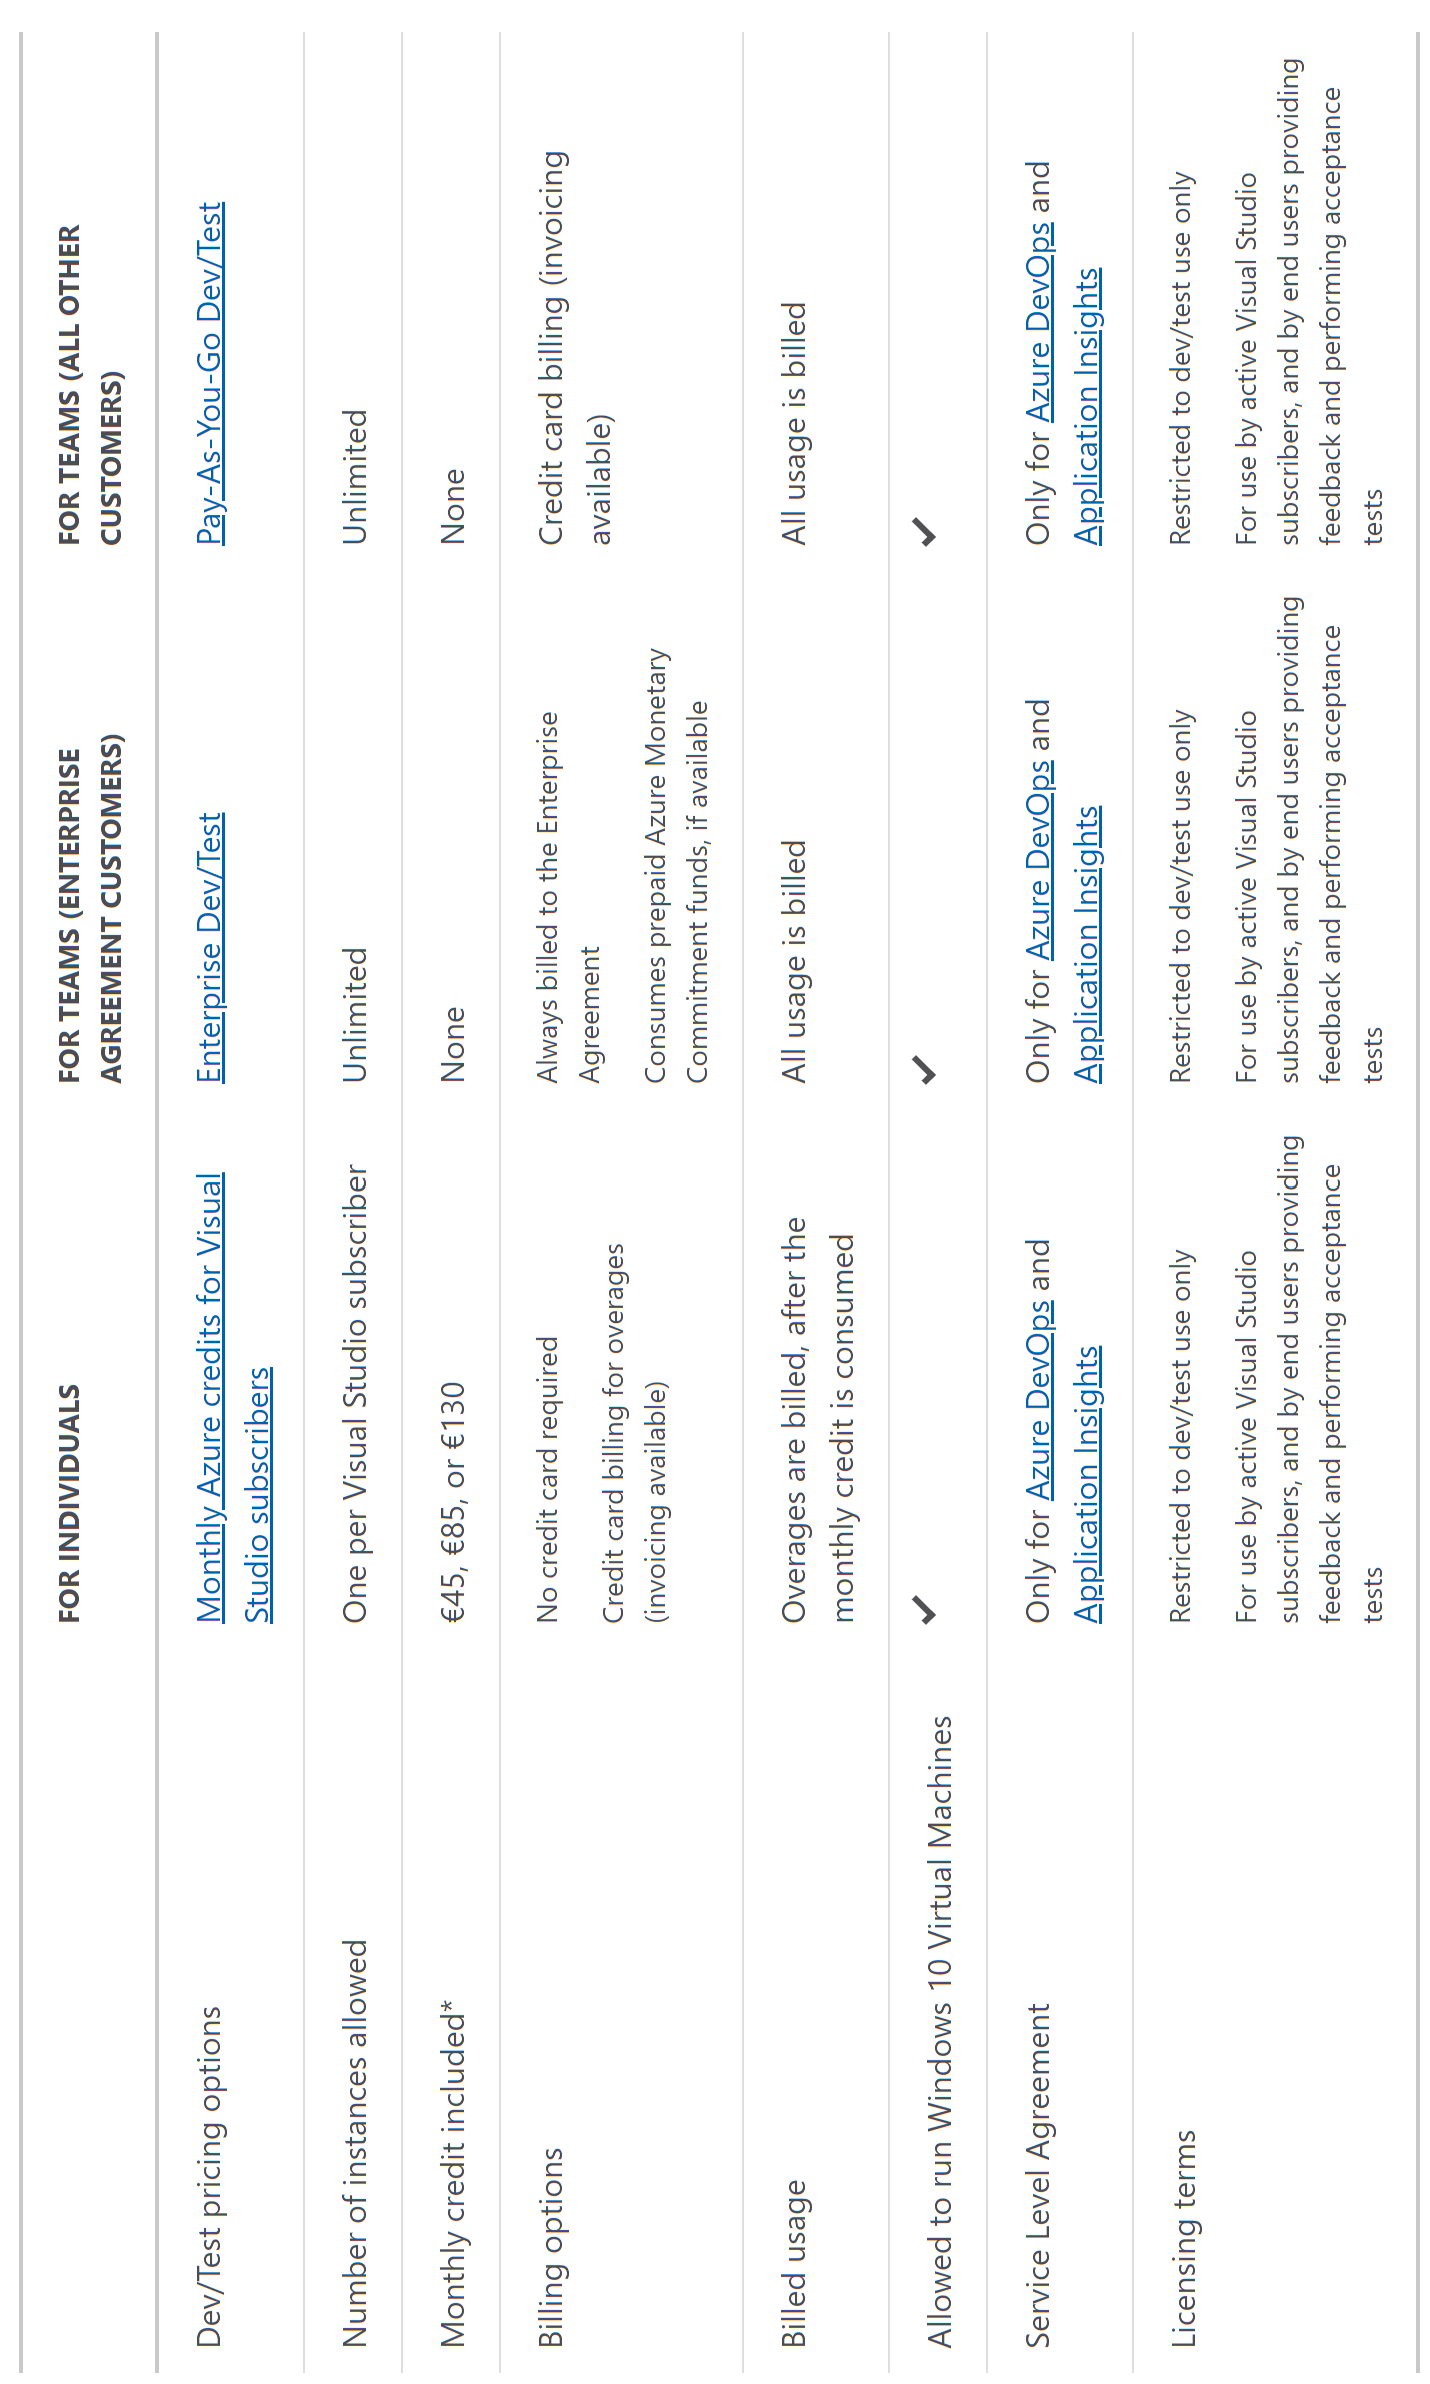
\includegraphics[width=\textwidth,height=\textheight,keepaspectratio]{../../Foto's/azure-pricing-tiers} 
	\captionsetup{justification=centering,margin=2cm}
	\caption{Azure Dev/Test prijzen. (\cite{Microsoft2020f})}
	\centering
\end{figure}

\subsection{Opzet API}
In de volgende sectie wordt de configuratie en opzet van een appservice, meer bepaald de Computer Vision API, in chronologische volgorde doorlopen en besproken. Hierbij wordt er inzicht gegeven in de mogelijke limitaties van de API en eveneens de verbonden transactiekosten. Na de opzet van deze API is het mogelijk om deze aan te roepen vanuit een software implementatie die in de volgende sectie besproken wordt. 


\newpage Een service kan men aanvragen via de Azure marketplace, hier wordt er een overzicht weergeven van de verschillende categorieën van services. De Computer Vision API valt onder de categorie: ‘AI + Machine Learning’ en wordt beschouwd als een Cognitieve Service. (\cite{Microsoft2020c}) 



De eerste stap is het navigeren naar de marketplace om vervolgens Computer Vision te selecteren. Na deze selectie krijgt men de optie aangeboden om een instantie van deze service aan te maken, gepaard gaande met de configuratie mogelijkheden zichtbaar op figuur 4.2   
\begin{figure}[h]
	
	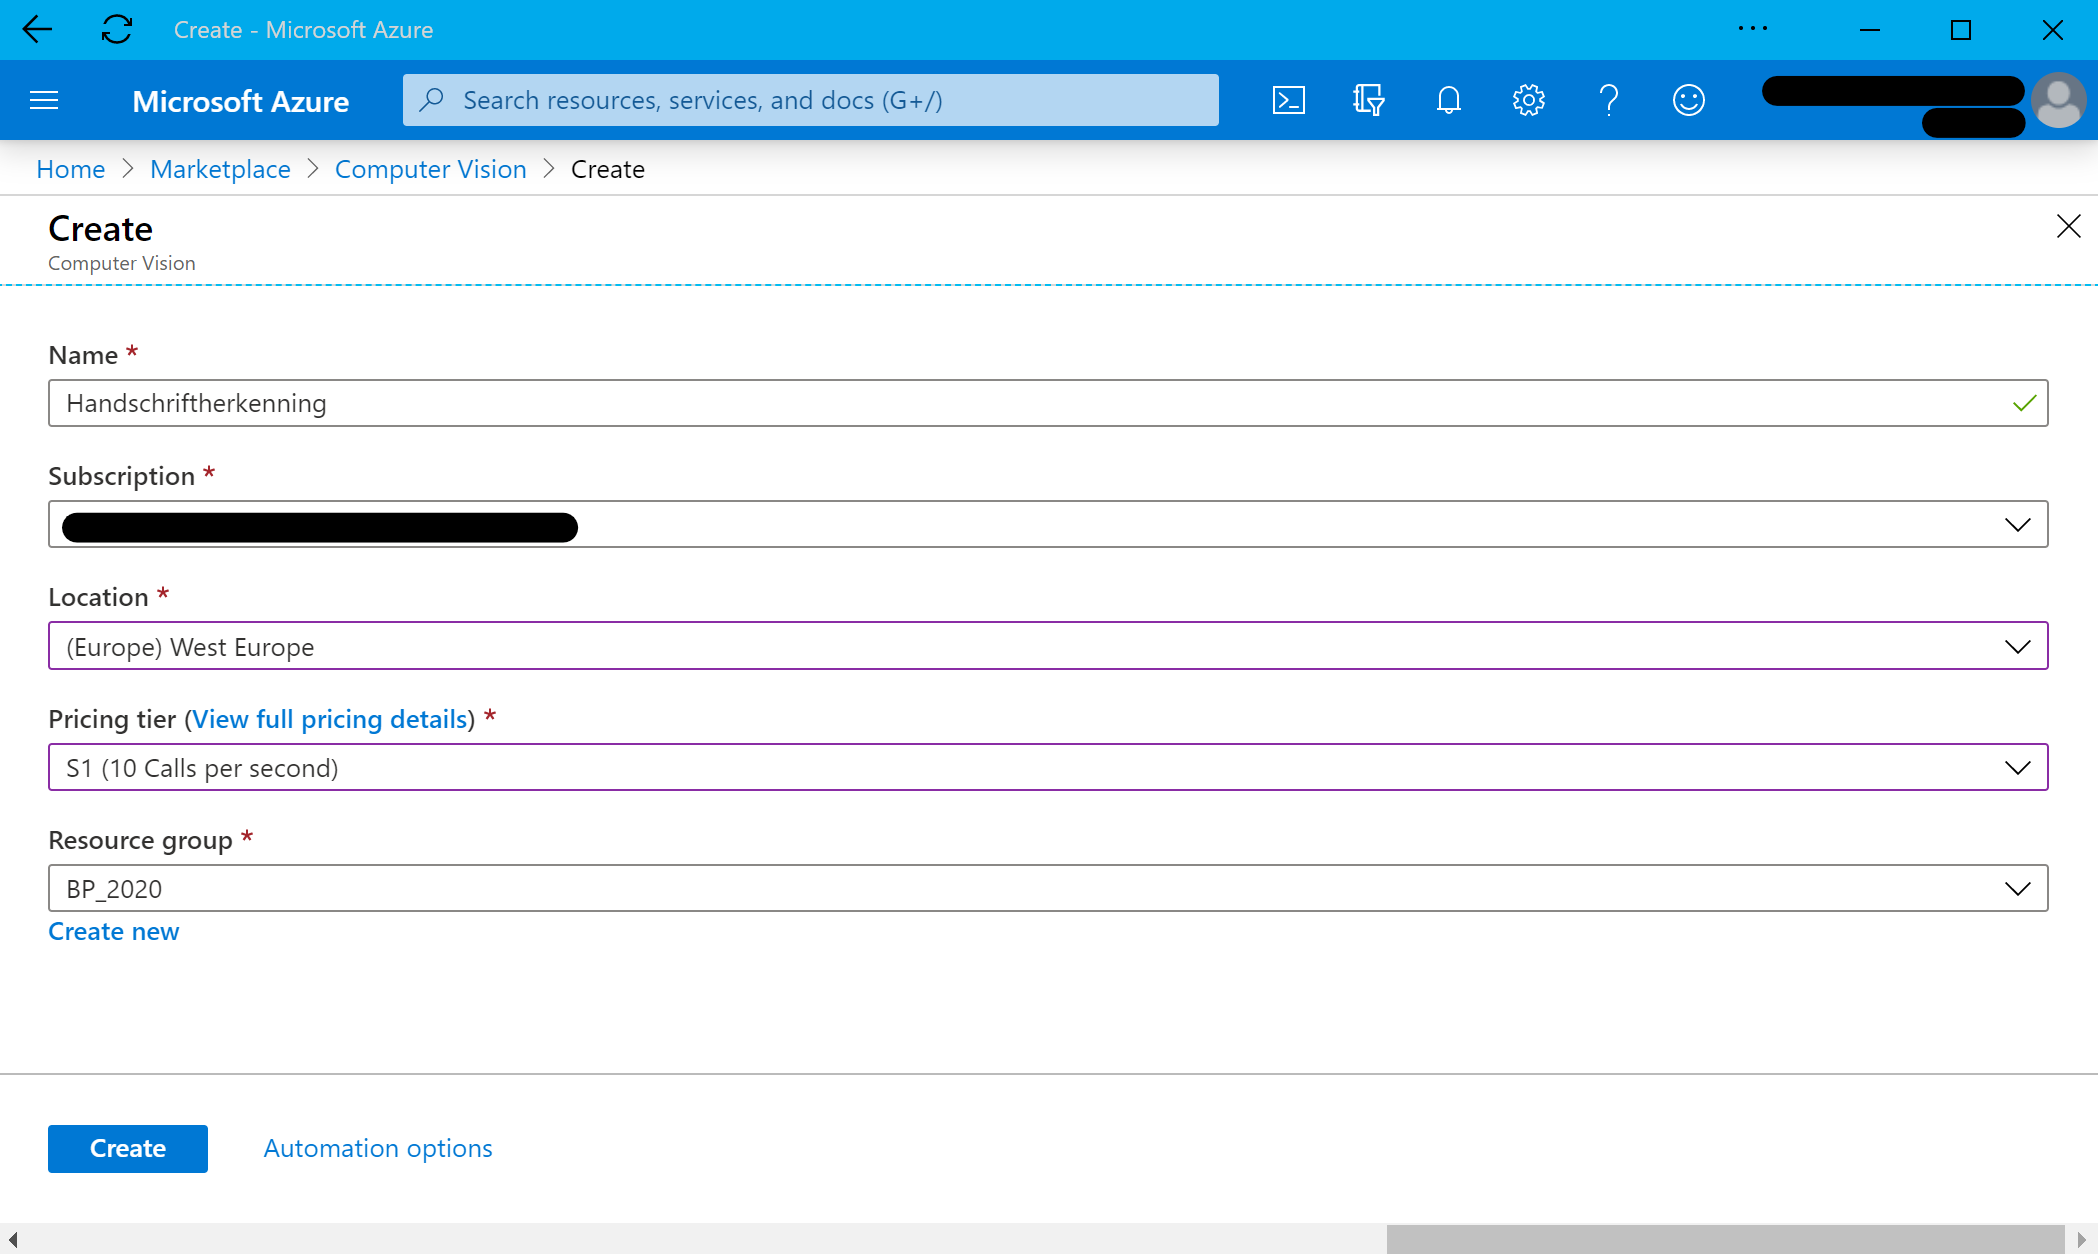
\includegraphics[width=\textwidth,height=\textheight,keepaspectratio]{../../Foto's/computer-vision-config}
	\captionsetup{justification=centering,margin=2cm}
	\caption{Computer Vision creatie pagina. }
	\centering
\end{figure}

De creatie van een Computer Vision instantie verwacht 5 parameters: 

\begin{itemize}
	\item \textbf{Name}
	\item \textbf{Subscription}
	\item \textbf{Location}
	\item \textbf{Pricing tier}
	\item \textbf{Resource group}
\end{itemize}
De naam van een instantie mag enkel bestaan uit alfanumerieke karakters en dient nog niet te bestaan binnen de geselecteerde resource groep. Verder dient de lopende subscriptie van de ingelogde gebruiker geselecteerd te worden. Indien parameters zoals “pricing tier” buiten de scope van de subscriptie gaan krijgt de gebruiker een melding dat de gekozen subscriptie niet volstaat voor de gekozen noden en dat een upgrade nodig is. De gekozen locatie speelt een belangrijke rol als het aankomt op latentie en response time van de API. Hierdoor ligt de beste keuze voor dit onderzoek bij de West-Europese endpoint. 
\newpage
De pricing tier komt in twee verschillende opties:  
\begin{itemize}
	\item \textbf{F0 (20 Calls per minuut)}
	\item \textbf{F1 (10 Calls per seconde)}
\end{itemize}

Beide pricing tiers bieden standaard interactie met de API aan en kan men enkel onderscheiden in het aantal toegelaten transacties per tijdseenheid. De F0 tier volgt een vereenvoudigt transactieplan aangezien dit gratis verkregen kan worden. Bij dit plan wordt er een maandelijkse limiet ingesteld van 5000 transacties samen met een call limiet van 20/minuut. Voor de meeste gebruikers die een niet commerciële actie verrichten, volstaat dit plan. Echter biedt de service ook de S1 tier aan die meer gericht is naar gebruik op Enterprise niveau. Er wordt hierbij voor het Read onderdeel van Computer Vision, een vaste prijs opgesteld van €2.109 per 1,000 transacties. (\cite{Microsoft2020g}) 

\begin{figure}[h]
	
	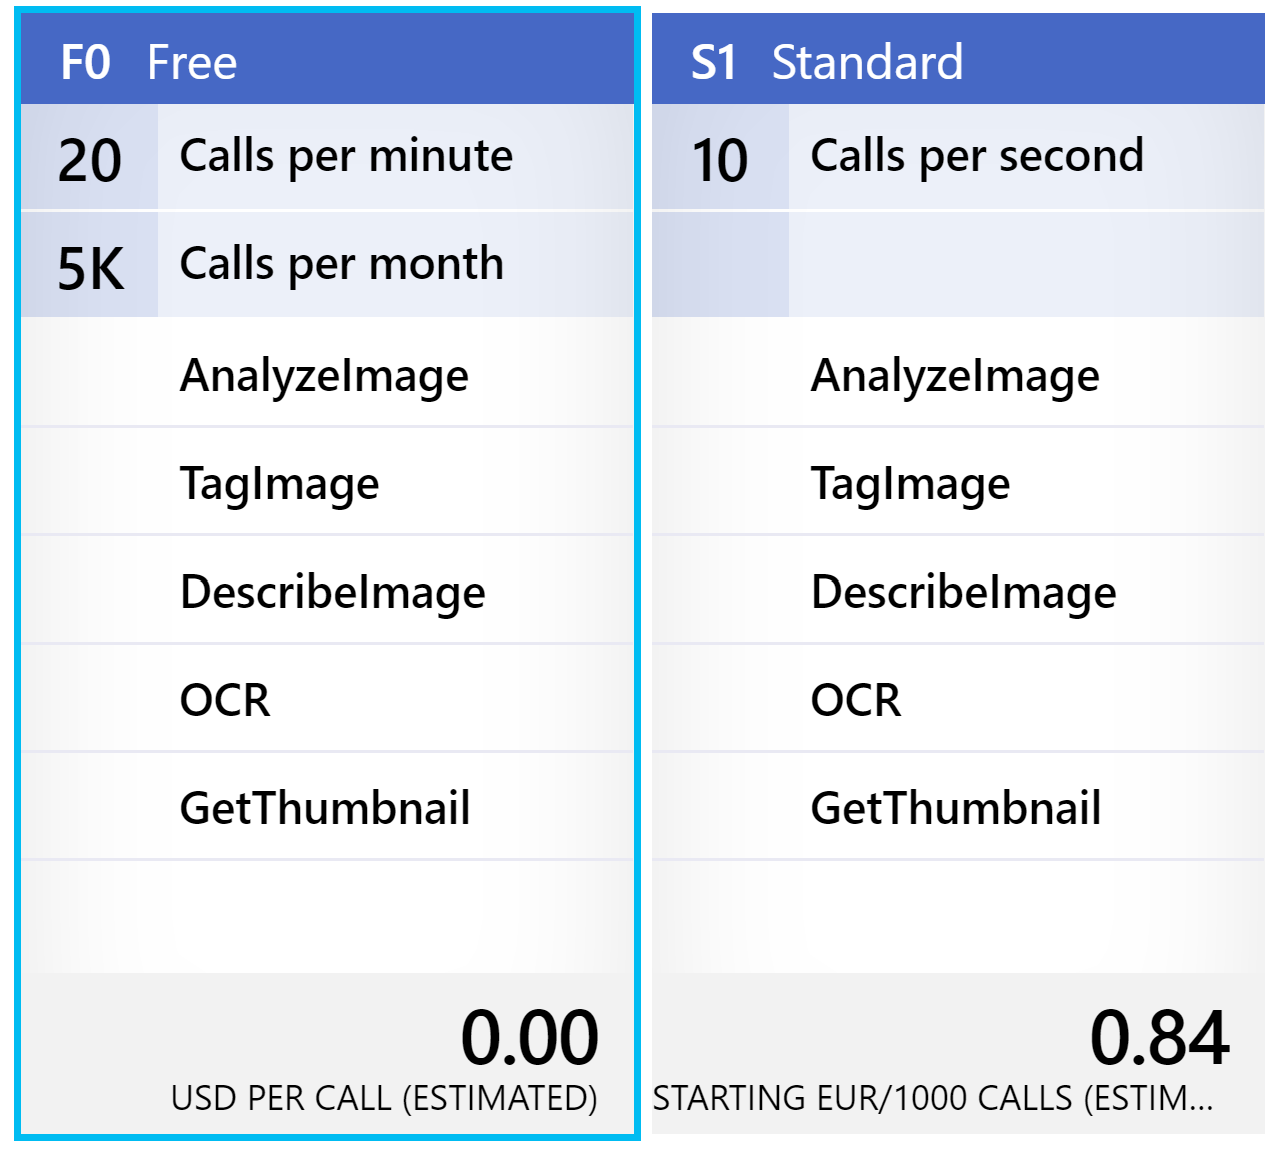
\includegraphics[width=\textwidth,height=\textheight,keepaspectratio]{../../Foto's/computer-vision-pricing}
	\captionsetup{justification=centering,margin=2cm}
	\caption{Pricing tier opties.}
	\centering
\end{figure}
Omdat dit een observatief onderzoek is, volstaat de F0 tier voor het uitvoeren van de test cases en het verzamelen van genoeg data om een conclusie te kunnen trekken. Verdere implementatie van de ontwikkelde software in een productie omgeving kan een hogere tier verwachten. Wanneer men opmerkt dat de F0 tier niet volstaat voor de implementatie, is het mogelijk deze achteraf te upgraden in het API-overzicht (zie fig 4.3). 



Na creatie van de service krijgt men een bevestiging mail toegestuurd met de verwachte uitrol tijd. Dit zou niet langer mogen duren dan 5 minuten. Eens beschikbaar, kan men de onderhoudspagina van de service terugvinden in het Azure dashboard. Hier zijn enkele belangrijke parameters van belang om de nodige communicatie te voorzien met software die calls naar de API verstuurd. Dit zijn namelijk de volgende parameters:  
 
\begin{itemize}
	\item \textbf{API Key }
	\item \textbf{API Endpoint}
\end{itemize}

Elke request uitgevoerd naar de API verwacht een geldige API key en zorgt ervoor dat deze request geautoriseerd wordt (\cite{Microsoft2019a}). Door deze key weet de API ook wat de limieten zijn van het gekozen plan. De API Endpoint is dan de uiteindelijke URL waar de request naar verstuurd wordt. De endpoint bevindt zich dan ook eveneens op de locatie gekozen bij configuratie van de service. De verdere implementatie en het gebruik van deze parameters wordt verder besproken in de volgende sectie.


Het is echter ook nog op te merken dat de huidige versie van de API (Version 3) enkel de extractie van Engels en Spaanse handgeschreven tekst ondersteunt.  Er is in dit onderzoek bewust gekozen om de extractie uit te voeren op Engels geschreven doktersbriefjes. Zoals besproken in hoofdstuk 3, is het verzamelen van handgeschreven teksten in het Nederlands een zeer moeilijke taak. Dit vergt in de meeste gevallen de samenwerking met een tweede partij die willend is om deze data vrij te geven. Daarom is er voor dit onderzoek zoals besproken in hoofdstuk 3, gekozen om gebruik te maken van een Cloud computing model dat getraind is met een generieke dataset. Dit is in zekere zin ook een interessante omgeving waar testen uitgevoerd kunnen worden. Deze testen kunnen aantonen of een generieke dataset even goed presteert bij de extractie van medische termen. In toekomstige versies en naarmate de evolutie van de API, zullen vermoedelijk meerdere talen ondersteunt worden voor extractie, waaronder Nederlands. 

De OCR API ondersteund momenteel wel al de extractie van geprinte tekst in het Nederlands samen met 25 andere talen (\cite{Microsoft2019b}). 


\subsection{Het gebruiken van de API}
De volgende sample code van deze implementatie is beschikbaar op  \href{https://github.com/Helmidyh/HD\_Bachelorscriptie\_Software\_2020}{github},  en werd grotendeels verkregen door \cite{Microsoft2020h} mits enkele aanpassingen voor string parsing. Vervolgens zullen de belangrijkste onderdelen van deze code besproken worden samen met een test request + resultaat. De code werd opgebouwd in C\# .NET en maakt gebruik van het Newtonsoft.Json framework voor eenvoudige interactie en manipulatie van Json bestanden. 
 

\subsection{Authenticatie} 

 

Zoals besproken in de voorgaande sectie, zal elke request verstuurd naar de API, geautoriseerd moeten worden. Dit houdt in dat de API Key meegegeven wordt in de hoofding van de request. Echter is het van enorm belang dat men beide Api Key en Endpoint nooit in code mag terugvinden en dit al zeker niet in een github of productie omgeving. Gebruikers die geen eigenaar zijn van de API kunnen met deze key ongezien requests versturen en data ontvangen. Men kan deze key op enkele manieren verbergen in het project, ook de mogelijkheid is er om gebruik te maken van Azure Keyvault. Hierbij wordt een gezamenlijk overzicht weergeven van al de beschikbare keys van het gebruikers account. Deze zijn achteraf raadpleegbaar met een request call naar de keyvault. 

 

In deze toepassing werd er gekozen om de parameters \textit{subscriptionKey} en \textit{endpoint}, temporeel op te slagen in de  omgevingsvariabelen van het project. Hierdoor worden deze enkel geïnjecteerd bij opstart en zijn ze deels verborgen. 
\newline



\codefragment{java}{parameters.cs}{}
	\textit{Fragment 1.1: Parameters.}


De \textit{uriBase} is een samengestelde parameter bestaande uit de gegenereerde API endpoint van de service, samen met het type request dat men wenst uit te voeren. In dit geval zal de \textit{read} operatie uitgevoerd worden.  

 
\subsection{Opbouwen van een request}
Een read request wordt vervolgens opgebouwd door het initialiseren van een HttpClient. Deze client voegt nodige parameters toe aan de request body en header, vooraleer men deze afvuurt. In fragment 1.2 wordt de API key toegevoegd aan de header. Dit is zoals besproken in sectie 4.0.3 nodig om de request te autoriseren. Verder is het van belang dat de taal van de meegegeven afbeelding gespecifieerd wordt. Momenteel is dit Engels in het formaat “en\_US”, maar in latere stages van de API zal dit evolueren naar Nederlands. 

\newpage
\lstinputlisting{request.cs}
\textit{Fragment 1.2: HttpClient.}




Uiteraard is het van belang dat een afbeelding meegegeven wordt aan de request. Men kan echter niet zomaar een “JPEG” of “PNG” meegeven aan de client. Deze dient eerst omgezet te worden naar een binaire voorstelling van data, in dit geval een array van bytes. Vervolgens wordt deze array van bytes meegegeven aan een instantie van “ByteArrayContent”. Deze instantie combineert de binaire data samen met het “MediaType” van de data. Hierdoor weet de API het type van de meegeleverde data in de body. 
\subsection{Versturen van een request}
Na opzet van de request header en body, kan men de “client” utiliseren om een post request te versturen m.b.v. de methode \textit{PostAsync()} (zie fragment 1.3). Deze methode ontvangt twee parameters, namelijk de “url” en de samengestelde “ByteArrayContent”. Merk op dat deze methode van het type Async is. Dit betekent dat men nooit zeker is wanneer men het beoogde resultaat terugkrijgt van de API en zal dit aldus asynchroon toekomen. 


Om onnodige fouten te vermijden wordt een “await” operator vóór de functie toegevoegd. Deze operator zorgt er voor dat verdere code afhankelijk is van het resultaat van deze response en blokkeert hierbij dus andere threads tót een resultaat verkregen is. 


Het geretourneerde resultaat bevat echter niet de geëxtraheerde tekst, maar één van twee status codes. Bij aanvang van een POST request, zal de API een read operatie uitvoeren op de meegeleverde afbeelding en vervolgens het bekomen resultaat bijhouden. Dit resultaat dient achteraf opgehaald te worden door wijze van een GET request naar de API. In fragment 1.3 wordt een check uitgevoerd op de geretourneerde statuscode. Indien deze van het type “succes” is, bevindt de URI locatie van de geëxtraheerde tekst zich in de header van de response.

\newpage
\lstinputlisting{sendrequest.cs}
\textit{Fragment 1.3: Post request.}


Eens de URI gekend is, wordt deze gebruikt om een GET request op te bouwen. Hierin bevindt zich het uiteindelijke resultaat van de tekst-extractie in JSON formaat. Zoals beschreven in de samplecode van \cite{Microsoft2020h} is de tijd van teruggave afhankelijk van de hoeveelheid te verwerken tekst. Daarom wordt aangetoond in fragment 1.4, dat om de 1000 ms een check gedaan wordt op de beschikbaarheid van de data. 




\lstinputlisting{sendrequest.cs}
\textit{Fragment 1.4: Get request.}

\subsection{Response}
Dit concludeert in grote lijnen de werking van de API, in de volgende sectie wordt een eenvoudige test request opgezet met een beter inzicht op wat voor data de API precies retourneert en hoe deze gebruikt kan worden in een probleem dat zich kan voordoen in de echte wereld. In eerste instantie zal dit een JSON-string zijn met een aantal zeer specifieke eigenschappen van elk gedetecteerd woord. 

Om dusdanig de software te gaan testen, wordt op figuur 4.4 gebruik gemaakt van een redelijk leesbaar doktersbriefje. Merk op dat deze voorschriften drastisch kunnen variëren en dat deze verschillende vormen kunnen aannemen.  
\begin{figure}
	\newpage
	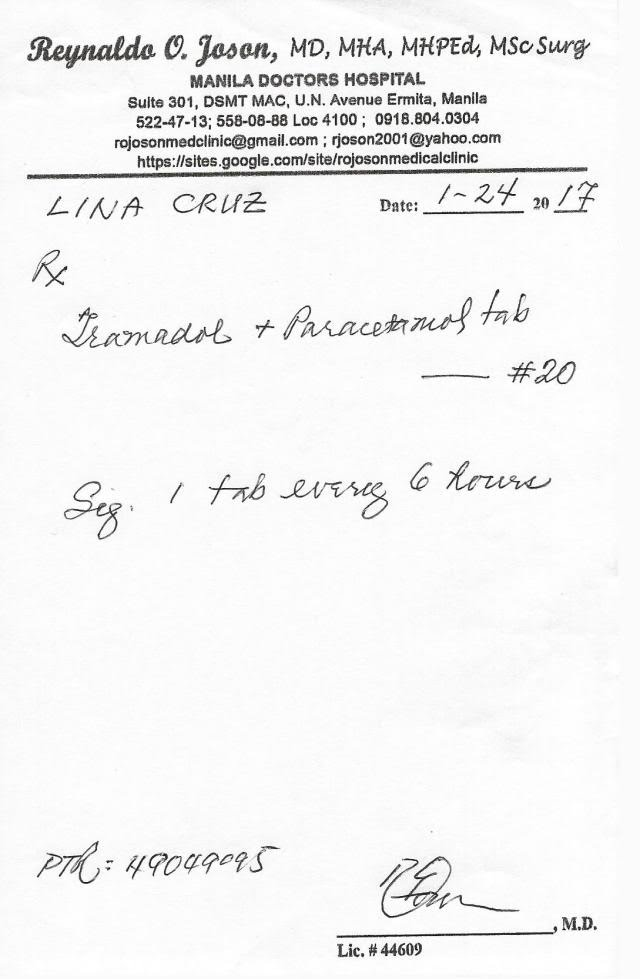
\includegraphics[width=\textwidth,height=\textheight,keepaspectratio]{../../Foto's/prescription_legible_roj_17jan24}
	\captionsetup{justification=centering,margin=2cm}
	\caption{Doktersbriefje voorbeeld. \cite{Joson2017}}
	\centering
\end{figure}


Een eerste uitdaging is dus om na te gaan of medische termen, meer bepaald medicatie zoals “Tramadol” en “Paracetamol” gezien in figuur 4.4, gedetecteerd worden. Dit zou enerzijds al een eerste stap zijn om een conclusie te trekken bij dit onderzoek. De volledige handgeschreven tekst die als persoon waargenomen wordt zou dus het volgende zijn:

\begin{itemize}
\item LINA CRUZ 
\item PX
\item Tramadol + Paracetamol tab 
\item  \#20 
\item Seg. 1 tab every 6 hours 
\item PTR : 49049095 
\end{itemize}

Vervolgens laten we de software los op figuur 4.4 en bekijken de uitkomst. Het ruwe JSON-resultaat is terug te vinden op \href{https://github.com/Helmidyh/HD\_Bachelorscriptie\_Software\_2020}{github} maar zal voor leesbaarheid geparsed worden naar een duidelijker resultaat. \cite{Microsoft2017} beschrijft de parameters in deze geretourneerde JSON als volgt: 

\begin{itemize}
\setlength\itemsep{1em}
\item \textbf{Status:} De teruggekeerde status van de request,  mogelijks “succeeded”, "notStarted", "failed" en "running". Vanaf deze status op "succeeded" komt te staan, zal het JSON-bestand de herkende tekst bevatten.  

\item \textbf{Lines:} Een lijst van herkende zinnen. Het maximum aantal lijnen dat op één pagina gedetecteerd kan worden is 300. Hierbij worden deze lijnen gesorteerd op de volgorde waarin deze gedetecteerd werden (van linksboven naar rechtsonder). De lijnen stellen dan in de meeste gevallen ook een volledige zin voor. 

\item \textbf{Text:} Een volledig herkende zin in één lijn, deze wordt verder opgesplitst in een lijst van woorden.

\item \textbf{Words:} Een verzameling van woorden in een herkende zin.

\item \textbf{BoundingBox:} Een rechthoek dat de positie bevat van de herkende zin of het herkende woord, gespecifieerd als een lijst bestaande uit 8 nummers. Deze nummers stellen de coördinaten van het herkende woord voor, relatief aan de linkerbovenhoek van de afbeelding. Dit zijn dus 4 paren van x,y coördinaten waardoor een rechthoek gevormd wordt (zie fragment 1.5). 

\item \textbf{Confidence:} Het vertrouwensniveau van elk gedetecteerd woord. Zoals beschreven in hoofdstuk 2, zou dit voor handgeschreven teksten lager moeten liggen dan getypte tekst. 
\end{itemize}

\newpage
Om in het volgende hoofdstuk collectief de resultaten op een eenvoudige wijze te vergelijken en samen te vatten, wordt dus gebruik gemaakt van een parsing methode. Deze methode genereerd een overzicht dat enkel de zin, de woorden en het vertrouwensniveau weergeeft, wat uiteraard ook de belangrijkste attributen zijn. 



In fragment 1.5 wordt een deel van het ruwe geretourneerde resultaat weergeven. Merk op dat voor de leesbaarheid, de “boundingBox” parameter van elk specifiek woord weggelaten is, aangezien men een algemene “boundingBox” van de volledige zin ter beschikking heeft. 

\lstinputlisting{rawresult.json}
\textit{Fragment 1.5: Ruw resultaat.}
\newpage
\lstinputlisting{parsedresult.txt}
\textit{Fragment 1.6: Parsed resultaat.}


Men kan duidelijk zien dat mits de lage vertrouwenswaarde, de zin “Tramadol + Paracetamol tab” volledig juist geëxtraheerd is. Dit resultaat stelt wel degelijk voor dat medische termen opgenomen zijn bij het trainen van het extractie model. Verder worden de rest van de handgeschreven zinnen vlekkeloos overgenomen. Dit toont enerzijds aan hoe accuraat dit model is mits dit nog een zeer recente technologie is.  


Als de gemiddelde accuraatheid genomen wordt van elk woord, denkt de API de tekst met een accuraatheid van 59\% voorspeld te hebben. In principe ligt dit percentage relatief laag aangezien men kan vaststellen dat de meerderheid van de woorden volledig juist voorspeld werden. Verder, was de responsetijd van de API was in dit geval +- 8.673 seconden. 

\subsection{Conclusie}
Uit dit hoofdstuk kunnen we concluderen dat het wel degelijk mogelijk is om handschrift te extraheren van een afbeelding. Dit enerzijds rekening houdend met medische termen en opschriften.  Wat nu momenteel echter in vraag gesteld wordt, is of dit resultaat aanhoudend is. Hoe reageert de API tegenover een ander type doktersbriefje, schrijfstijl of kleur? Het is onmogelijk om duizenden testen op te zetten om elke specifieke karakteristiek dat in een doktersbriefje kan voorkomen, te testen. 

In het volgende hoofdstuk worden enkele van deze algemeen gerichte vragen in een test gegoten. 
\chapter{Test cases}

Uit het vorige hoofdstuk kon men vaststellen dat de Computer Vision API wel degelijk een bruikbaar resultaat levert. Dit resultaat kan verder gemanipuleerd worden voor verscheidene use cases die zich kunnen voordoen in eender welk domein. In figuur 3.4 van hoofdstuk 4 werd een semi leesbaar doktersbriefje gebruikt. In principe was dit een perfect voorbeeld om enkel de functionaliteit van de API te testen. Echter is het van belang om na te gaan waar de API de lijn trekt.  



Om die redenen werden er in het volgende hoofdstuk drie test cases opgesteld. Elke van deze test cases bestaat uit één of meerdere doktersbriefjes. Hierbij werden deze voorgesteld aan aantal personen om na te gaan hoe zij deze tekst interpreteerden. Achteraf werd van elk geïnterpreteerd woord de populairste interpretatie genomen en vergeleken met het resultaat van de API.  

Hierdoor is het mogelijk om een rechtstreekse vergelijking uit te voeren van hoe mensen een onleesbare tekst interpreteren vergeleken met een AI-toepassing. 

Eveneens wordt er per extractie een tabel opgesteld met het geëxtraheerde woord, de interpretatie en de herkenningsgraad. 
\newpage
\section{Test Case 1}
\subsection{Opzet}
De eerste test case zal nagaan wat het effect van een verlaagde resolutie is op de extractie. Om dit effectief te gaan testen zal men gebruik maken van hetzelfde doktersbriefje in figuur 4.4 

Echter werd een kwaliteitscompressie op deze afbeelding uitgevoerd waarbij deze nog maar 60 \% van de originele kwaliteit bevat (zie fig 5.2). Vooraleer een vergelijking kan plaatsvinden, werd een statistische tabel van de originele extractie request opgesteld in figuur 5.1. Men kan duidelijk vaststellen dat de meerderheid van de woorden correct voorspeld werden.  

\begin{figure}[h]
	
	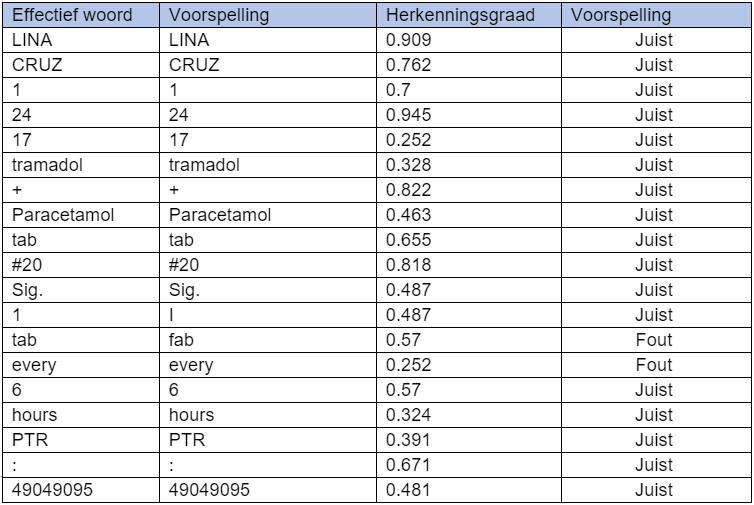
\includegraphics[width=\textwidth,height=\textheight,keepaspectratio]{../Foto's/doktersbriefje0_tabel}
	\captionsetup{justification=centering,margin=2cm}
	\caption{Doktersbriefje voorbeeld statistiek  100\% kwaliteit. \cite{}}
	\centering
\end{figure}
\subsection{Doktersbriefje verlaagde kwaliteit resultaat}
Wanneer naar figuur 5.2 gekeken wordt, ziet men op het eerste zicht visueel geen grote verschillen in kwaliteit, echter kan dit wel een invloed hebben op de extractie kwaliteit. Meer bepaald de virtuele “ruis”. Deze ruis kan karakters vervormen en in extreme gevallen deze zelfs onherkenbaar maken. Vervolgens werd er een extractie request afgevuurd op figuur 5.2 en werd de verkregen data hiervan in tabel 5.3 weergegeven.
\begin{figure}[h]
	
	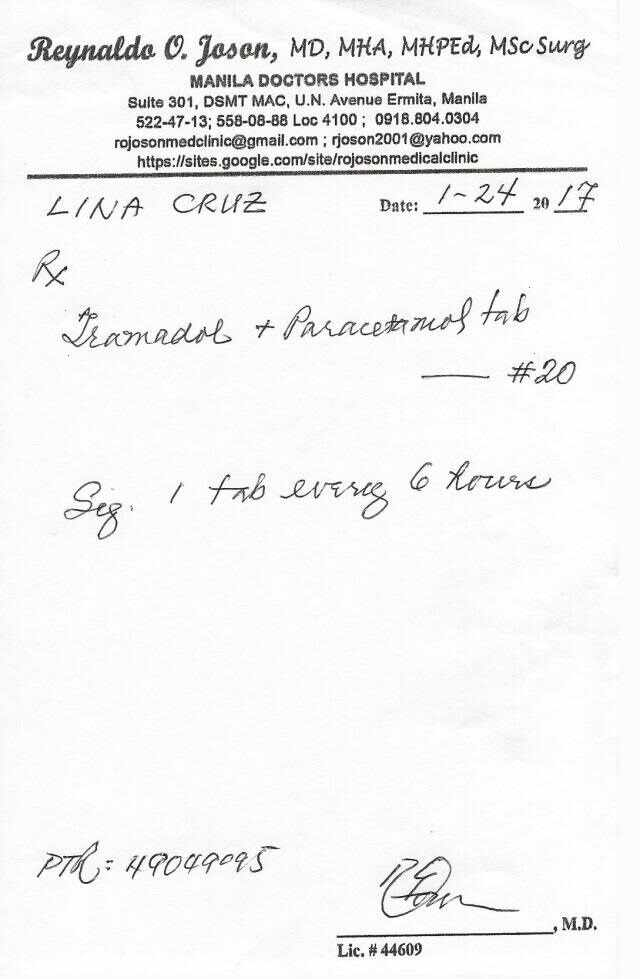
\includegraphics[width=\textwidth,height=\textheight,keepaspectratio]{../doktersbriefjes/61procent}	
	\captionsetup{justification=centering,margin=2cm}
	\caption{Doktersbriefje voorbeeld 60\% kwaliteit. \cite{}}
	\centering
\end{figure} 

\clearpage
\begin{figure}[h]
	
	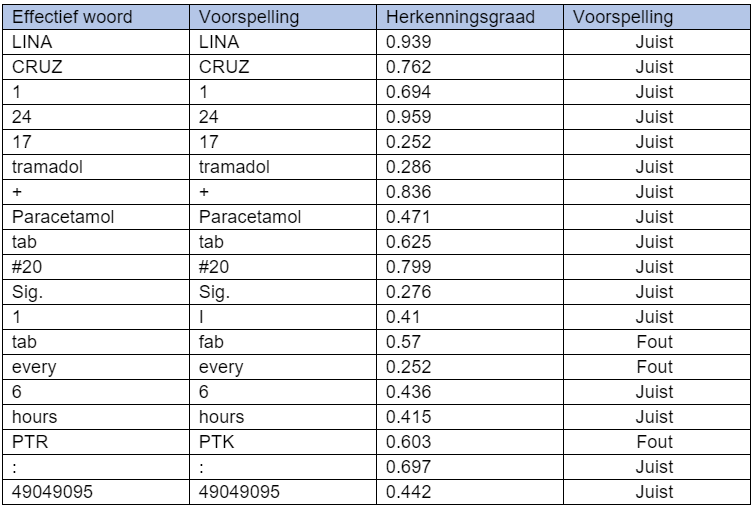
\includegraphics[width=\textwidth,height=\textheight,keepaspectratio]{../Foto's/doktersbriefje0_60procent_tabel}
	\captionsetup{justification=centering,margin=2cm}
	\caption{Doktersbriefje voorbeeld statistiek 100\% kwaliteit. \cite{}}
	\centering
\end{figure}


Wanneer men beide tabellen vergelijkt zijn er enkele verschillen die meteen naar voor komen. Zoals verwacht is de algemene herkenningsgraad gedaald. De meerderheid van de woorden werden nog steeds juist voorspeld echter met een lagere herkenningsgraad. Er werd één woord vergeleken met figuur 4.4 verkeerd voorspeld, namelijk "PTR". Dit stelt voor dat een lagere resolutie wel degelijk invloed kan hebben op de extractie. Narmate de verlaging in kwaliteit zullen meer en meer woorden verkeerd voorspeld worden.



\section{Test Case 2}
\subsection{Opzet}
De tweede test case is een meer generiek gerichte test, hierbij wordt gekeken naar de algemene accuraatheid van de teruggegeven data en het aantal juiste voorspellingen. Hier werd een andere aanpak genomen tegenover test case 1. De juistheid wordt hierbij bepaald door de voorspelling te vergelijken met een interpretatie. Hierbij werden vier doktersbriefjes voorgesteld aan een groep mensen. Elke persoon in deze groep probeerde de handgeschreven tekst in deze doktersbriefjes zo accuraat mogelijk te interpreteren.  Achteraf werd de gemiddeld populairste interpretatie van elk woord genomen en in een tabel gegoten. Door een vergelijking uit te voeren van het voorspelde met de interpretatie, kan men nagaan of de API handgeschreven woorden op dezelfde manier interpreteert als mensen. 
%%=============================================================================
\subsection{Doktersbriefje 1 resultaat}
Zoals men kan zien op figuur 5.4 zijn er in totaal 23 woorden/karakters geëxtraheerd. Hierbij zijn 14 van deze 25 correct voorspeld naargelang de interpretatie. Merk op dat men de interpretatie niet als volledig betrouwbaar mag beschouwen. Een persoon kan zonder medische achtergrond of kennis een woord op een volledig andere manier interpreteren dan iemand die ervaring heeft in dit domein. Een voorbeeld hiervan zijn de woorden “amoxicillin” en “Himox”, de populairste interpretatie hiervan werd gezien als “omoxirillin” en “Hinlox”.  


Echter kan men deze voorspelling niet zoals in andere gevallen fout beschouwen, want “amoxicillin” en “Himox” zijn medisch correcte termen. Men kan dus wel degelijk vaststellen dat medische termen in hun geheel correct voorspeld kunnen worden, echter is hier wel nog een manuele controle voor nodig.  In conclusie kan men een gemiddelde herkenningsgraad van 0.45087 per woord vinden, met 60\% van deze woorden correct voorspeld. 
\begin{figure}[h]
	
	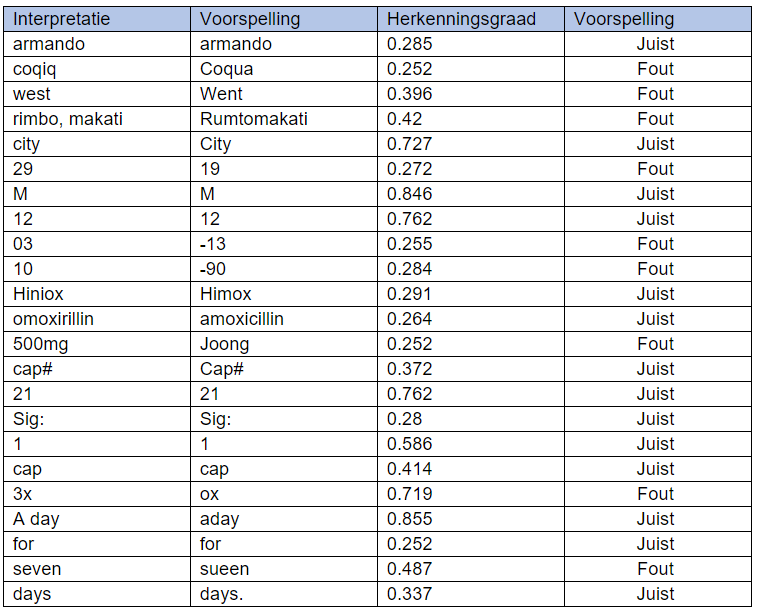
\includegraphics[width=\textwidth,height=\textheight,keepaspectratio]{../Foto's/doktersbriefje1_tabel}
	\captionsetup{justification=centering,margin=2cm}
	\caption{Doktersbriefje 1 extractie resultaat}
	\centering
\end{figure}
\clearpage
\begin{figure}
	
	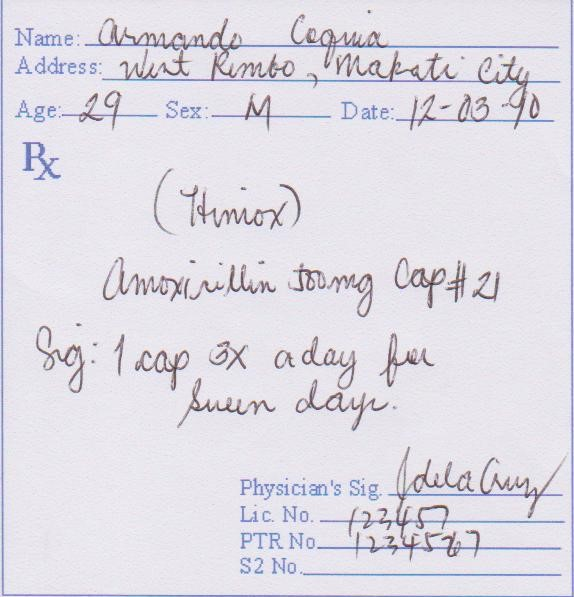
\includegraphics[width=\textwidth,height=\textheight,keepaspectratio]{../doktersbriefjes/dokterbriefje_1.jpg}
	\captionsetup{justification=centering,margin=2cm}
	\caption{Doktersbriefje 1. (\cite{Tacio2013})}
	\centering
\end{figure}
\clearpage
%%=============================================================================

%%=============================================================================
\subsection{Doktersbriefje 2 resultaat}
Bij de resultaten van de extractie op figuur 5.7 zijn er in totaal 22 woorden geëxtraheerd, waarvan 2 onbepaald. Eveneens zijn bij de interpretatie 3 woorden als onbepaald verklaard. Dit fenomeen doet zich voor wanneer bepaalde woorden onherkenbaar zijn voor de API, waardoor deze overgeslagen worden. Dit was dus het geval bij de interpretatie van “biovik 100 mg tab”. 


Een mogelijke oorzaak kan zijn dat 2 woorden te dicht bij elkaar staan of dat de gebruikte inkt mogelijks te licht is. Verder werden bepaalde woorden simpelweg oninterpreteerbaar verklaard door de testgroep, waardoor deze niet zullen bijdragen tot het gehele resultaat. De gemiddelde herkenningsgraad mits onbepaalde woorden is 0.525182, met 58 \% van de voorspelde en geïnterpreteerde woorden correct voorspeld. 
\begin{figure}[h]
	
	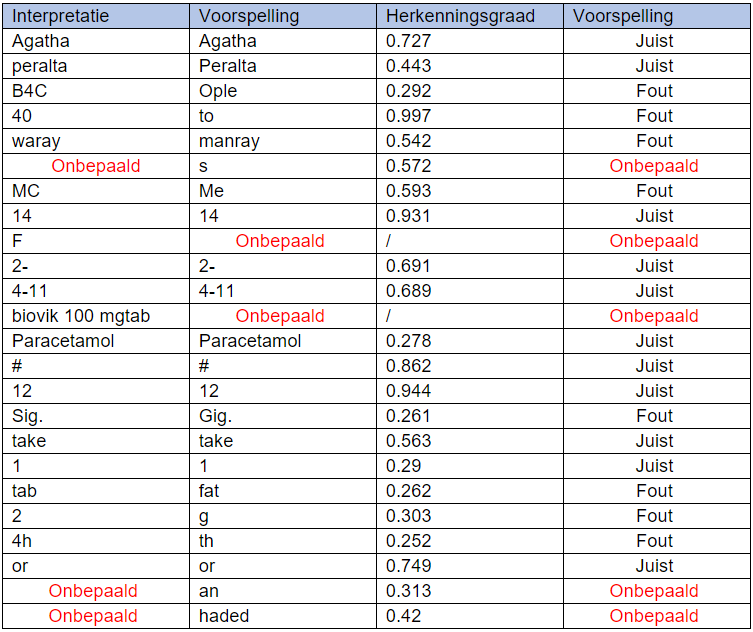
\includegraphics[width=\textwidth,height=\textheight,keepaspectratio]{../Foto's/doktersbriefje2_tabel}
	\captionsetup{justification=centering,margin=2cm}
	\caption{Doktersbriefje 2 extractie resultaat}
	\centering
\end{figure}
\clearpage
\begin{figure}
	
	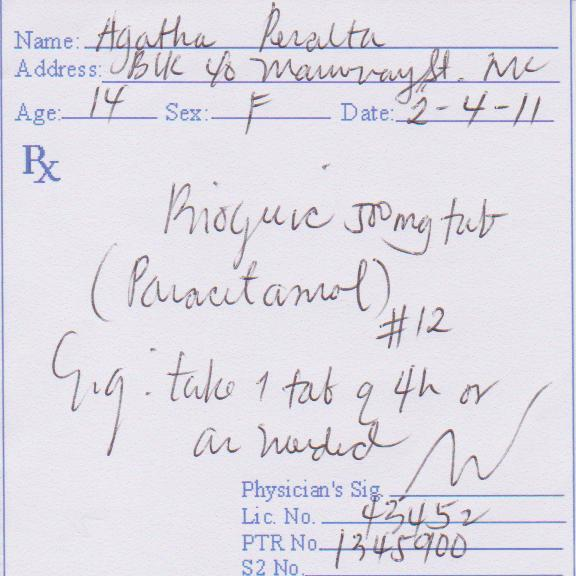
\includegraphics[width=\textwidth,height=\textheight,keepaspectratio]{../doktersbriefjes/dokterbriefje_2.jpg}
	\captionsetup{justification=centering,margin=2cm}
	\caption{Doktersbriefje 2. (\cite{Tacio2013})}
	\centering
\end{figure}
\clearpage
%%=============================================================================

%%=============================================================================
\subsection{Doktersbriefje 3 resultaat}
Volgens de resultaten van de extractie op figuur 5.9 zijn er in totaal 21 woorden geëxtraheerd, waarvan 1 onbepaald. Tegenover extractieresultaat 5.6 zijn hier veel minder woorden als onbepaald verklaard. Dit lijkt in zeker zin ook logisch als men kijkt naar de algemene slordigheid van figuur 5.7 vergeleken met figuur 5.9 Een terugkerende trend die men kan waarnemen bij deze resultaten, is de voorspelling van de medicatie dosering.  

Deze is in geen enkel van de gevallen tot nu toe juist voorspeld. De gemiddelde herkenningsgraad mits 1 onbepaald woord is 0.507048 met 57 \% van de voorspelde en geïnterpreteerde woorden correct voorspeld. 
\begin{figure}[h]
	
	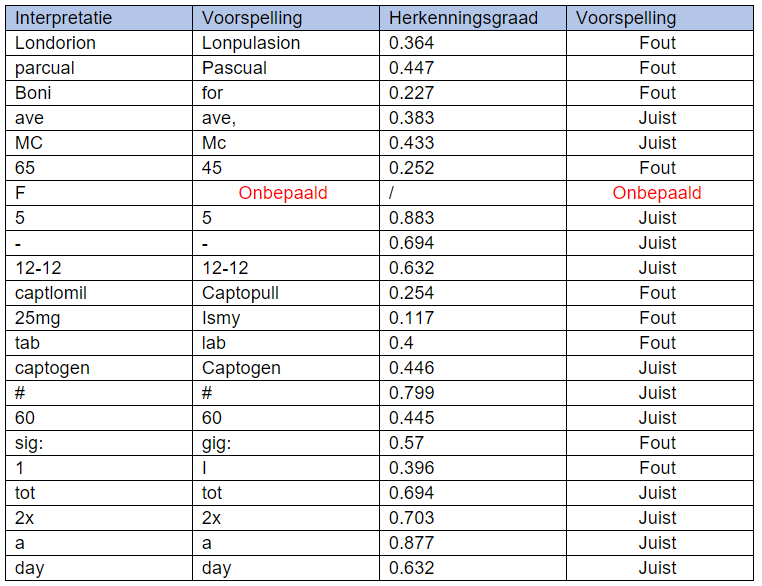
\includegraphics[width=\textwidth,height=\textheight,keepaspectratio]{../Foto's/doktersbriefje3_tabel}
	\captionsetup{justification=centering,margin=2cm}
	\caption{Doktersbriefje 3 extractie resultaat}
	\centering
\end{figure}
\clearpage
\begin{figure}
	
	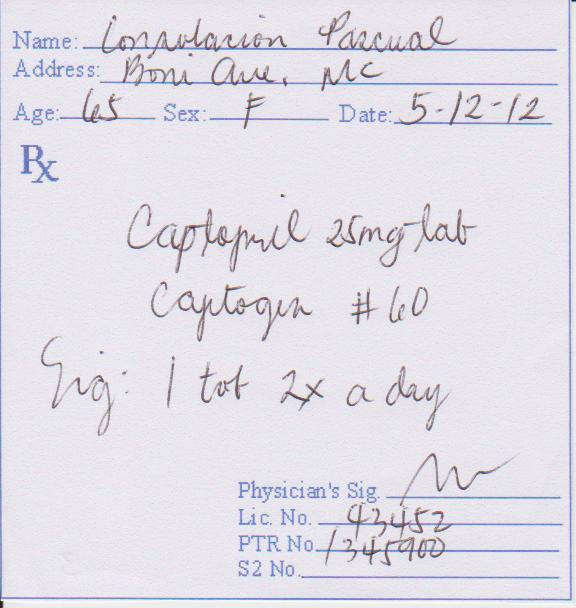
\includegraphics[width=\textwidth,height=\textheight,keepaspectratio]{../doktersbriefjes/dokterbriefje_3.jpg}
		\captionsetup{justification=centering,margin=2cm}
	\caption{Doktersbriefje 3. (\cite{Tacio2013})}
	\centering
\end{figure}
\clearpage
%%=============================================================================

%%=============================================================================
\subsection{Doktersbriefje 4 resultaat}
Bij de laatste extractie request ziet men positieve resultaten. Hierbij zijn 27 woorden geëxtraheerd, zonder onbepaalde voorspellingen. Merk op dat de meerderheid van de foutief gerekende voorspellingen, maar 1 karakter verschillen van de interpretatie. 


Een toekomstige oplossing voor dit probleem zou een fuzzy matching NLP model kunnen zijn. Hierbij worden woorden die enkele karakters van het originele afwijken, vergeleken met een generieke databank. Men kan op deze manier woorden die niet volledig juist verklaard zijn toch nog goedkeuren door wijze van vergelijking. Echter zou dit uiteraard de kost en tijd van extractie enkel maar vergroten. Kijkend naar het resultaat, werd er een gemiddelde herkenningsgraad van 0.564259 per woord bekomen, waarbij  64\% van de interpretatie correct voorspeld. 
\begin{figure}[h]
	
	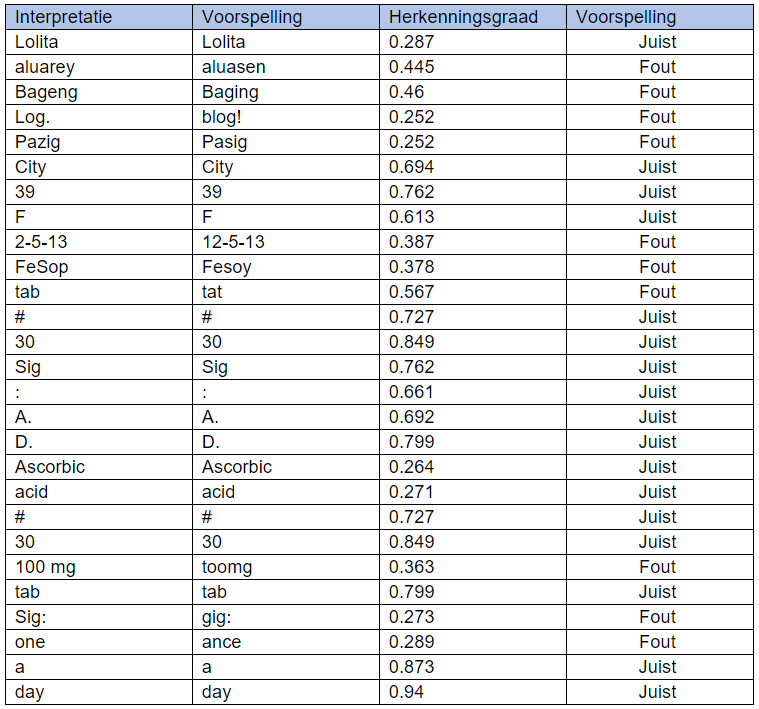
\includegraphics[width=\textwidth,height=\textheight,keepaspectratio]{../Foto's/doktersbriefje4_tabel}
	\captionsetup{justification=centering,margin=2cm}
	\caption{Doktersbriefje 4 extractie resultaat}
	\centering
\end{figure}
\clearpage
\begin{figure}
	
	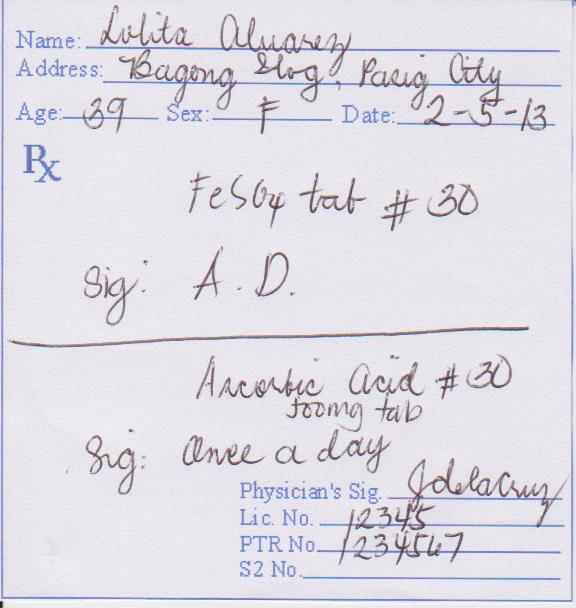
\includegraphics[width=\textwidth,height=\textheight,keepaspectratio]{../doktersbriefjes/dokterbriefje_4.jpg}
	\captionsetup{justification=centering,margin=2cm}
	\caption{Doktersbriefje 4. (\cite{Tacio2013})}
	\centering
\end{figure}
\clearpage
%%=============================================================================

\section{Test Case 3}
\subsection{Opzet}
De derde en laatste test case zal nagaan of het uiterlijk van een doktersbriefje invloed heeft op het gemiddelde resultaat. Voorgaande doktersbriefjes gebruikt in test case 2, maakten gebruik van éénzelfde template. Men bekomt hierdoor een gestroomlijnd resultaat waarbij men de uitkomst enkel kan baseren op het handgeschrift. Echter is het wel nog interessant om een extractie uit te voeren op een doktersbriefje dat gebruik maakt van een ander template. Hierbij wordt de positionering en volgorde van extractie mogelijks anders opgenomen door de API. 
Bij deze test werd gebruik gemaakt van het doktersbriefje weergeven in figuur 5.13. Merk op dat meerdere karakteristieken van figuur 5.13 duiden op een suboptimale extractie. Hierbij ziet men net zoals in test case 1, een lage resolutie gepaard met een slordig handschrift. In essentie stelt deze test een extreem geval voor dat zelden zal voorkomen bij een echte implementatie. 

\subsection{Doktersbriefje 5 resultaat}
Kijkend naar de resulterende data zichtbaar of figuur 5.12, kan men vaststellen dat de gemiddelde herkenningsgraad 0.496833 bedraagt. In totaal werd 50 \% van de interpretaties correct voorspeld door de API. Dit wijst m.a.w. op een daling van +- 8 \% tegenover de voorgaande resultaten. De meerderheid van de medische termen zijn hierbij wel correct voorspeld, met de tot nu toe enige correcte voorspelling van de medische dosering. 
\begin{figure}[h]
	
	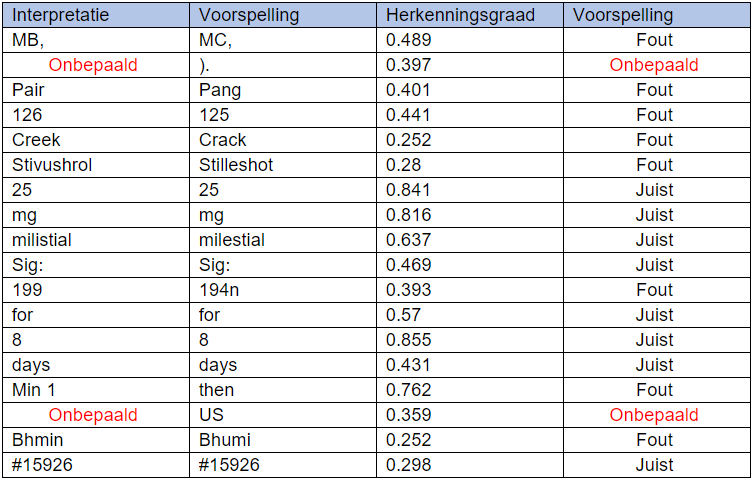
\includegraphics[width=\textwidth,height=\textheight,keepaspectratio]{../Foto's/doktersbriefje5_tabel}
		\captionsetup{justification=centering,margin=2cm}
	\caption{Doktersbriefje 5 extractie resultaat}
	\centering
\end{figure}
\clearpage
\begin{figure}
	
	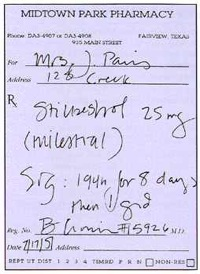
\includegraphics[width=\textwidth,height=\textheight,keepaspectratio]{../doktersbriefjes/dokterbriefje_5.jpg}
		\captionsetup{justification=centering,margin=2cm}
	\caption{Doktersbriefje 5. (\cite{Abrahams2008})}
	\centering
\end{figure}
\clearpage
\section{Resultaten}
Na het uitvoeren van de tests, kunnen we collectief de resultaten verzamelen en vergelijken.  
\subsection{Test cases}
Op figuur 5.14 ziet men een weergave van de bekomen extractie percentages.  Kijkend naar test 1, werd 84 \% van de geëxtraheerde woorden correct voorspeld. Vergeleken met de percentages bekomen in test case 2 en 3, ligt dit relatief hoog. Een mogelijke verklaring voor dit hoge percentage zou kunnen liggen bij de ruimere spreiding van de woorden op figuur 5.2.  



Extracties 2-5 uitgevoerd in test case 2, tonen een relatief gelijkaardig resultaat. Bij deze test case werden 4 doktersbriefjes met éénzelfde template getest. Gemiddeld werd 59.75 \% van de woorden correct voorspeld. De meerderheid van de foutieve voorspellingen lag bij de naam of het adres van de persoon in kwestie. In principe was dit te verwachten aangezien de focus bij de dataset minder ligt op unieke naamgevingen. Wat men echter wel kan vaststellen is dat de meerderheid van de medische termen correct voorspeld werden, wat bijdrage levert aan een positief resultaat. 



Test case 3 toonde, vergelijkend met test case 2, relatief weinig tot geen verschil aan in resultaat. Dit geeft enerzijds ook aan dat het uiterlijk van een doktersbriefje het resultaat niet ongewild beïnvloedt. Wat echter wel een tegenargument voor deze bewering kan zijn is dat de spreiding van de woorden, gezien bij doktersbriefje 1, bekomen werd door een groter schrijfvlak. Wat op zijn beurt weer een beter resultaat zou geven. 




 

\begin{figure}[h]
	
	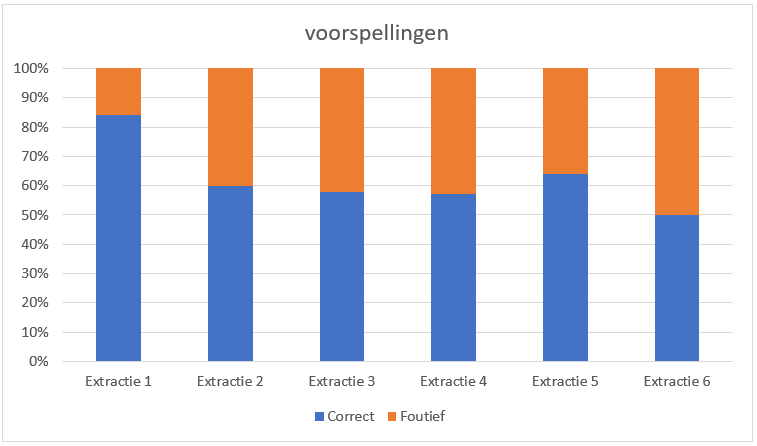
\includegraphics[width=\textwidth,height=\textheight,keepaspectratio]{../Foto's/voorspellingen_statistiek.png}
		\captionsetup{justification=centering,margin=2cm}
	\caption{Statestiek voorspellingen.}
	\centering
\end{figure}
 \clearpage
\subsection{Herkenningsgraad}
Verder, werd in figuur 5.15 het verloop van de herkenningsgraad per geëxtraheerd woord weergeven. Elke weergeven lijn stelt de volgorde voor waarin elk woord voorspeld werd, waarbij de y-as de zekerheid van extractie in \% voorstelt. Zoals eerder beschreven, ligt de meerderheid van foutieve voorspellingen bij de extractie van naam of adres. De oorzaak hiervan zou enerzijds liggen bij gebrek aan opname van unieke naamgevingen bij de training van het model. 


Merk op dat men dit fenomeen duidelijk kan waarnemen in figuur 5.15. De naam en adres van de patiënt worden in de meeste gevallen en dus ook bij de gebruikte doktersbriefjes bovenaan weergeven. Aangezien in hoofdstuk 4 (sectie 4.0.6) beschreven werd dat de API, een lijn extractie van linksboven naar rechtsonder uitvoert, zullen deze dus eerst geëxtraheerd worden. Men ziet ook wel degelijk dat de eerste 4-5 woorden bij elke extractie zelden een herkenningsgraad boven de 50 \% hebben.


\begin{figure}[h]
	
	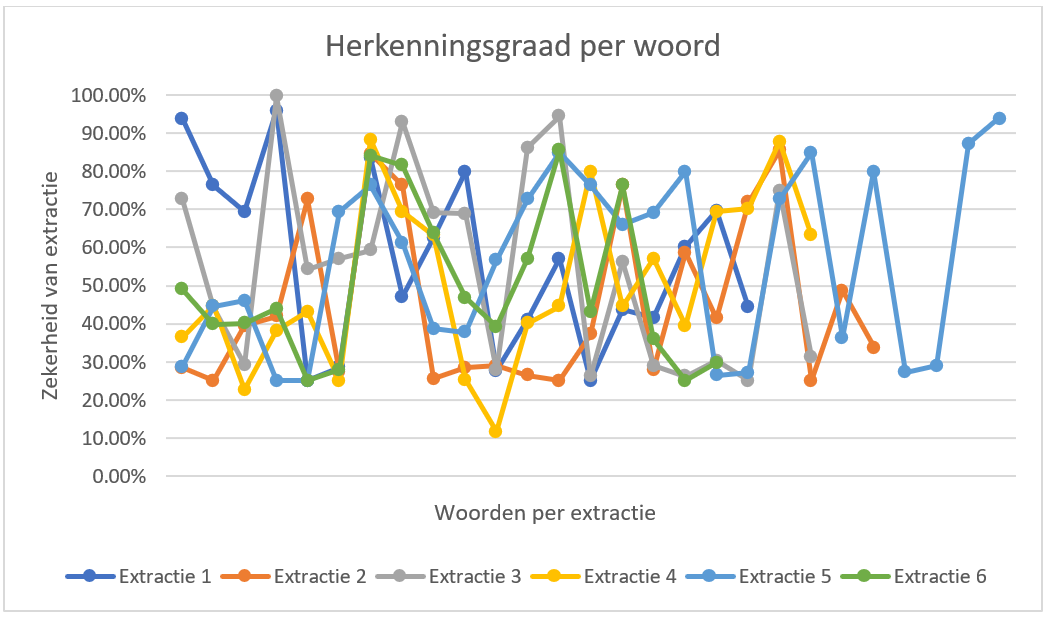
\includegraphics[width=\textwidth,height=\textheight,keepaspectratio]{../Foto's/herkenningsgraad_statistiek.png}
		\captionsetup{justification=centering,margin=2cm}
	\caption{Verloop van de herkenningsgraad per extractie.}
	\centering
\end{figure}

Collectief was de API bij het uitvoeren van de 3 test cases, per woord, gemiddeld 52 \% zeker van zijn voorspelling. Dit getal zal uiteraard evolueren, naargelang het aantal testen dat men uitvoert, vergroot en de variatie van het type doktersbriefjes toeneemt. 
\newpage
\section{Conclusie}
Uit de resultaten kon men vaststellen dat de Computer Vision API wel degelijk bruikbaar is voor het extraheren van doktersgeschrift. Hierbij werd de meerderheid van de woorden correct voorspeld, gepaard met de juiste medische termen. De interpretaties verzameld door de testgroep werden grotendeels ook door de API voorspeld. Het is echter wel op te merken dat bij deze tests maar een beperkt aantal doktersbriefjes gebruikt werd. Dit komt grotendeels door de beperkte beschikbaarheid en vrijstelling van dit type document. Uiteraard zijn de meeste mensen niet bereid om hun naam en gegevens open te stellen aan een breder publiek. Aangezien het bekomen van test cases al een moeilijke zaak was zou dit al zeker een hindernis vormen bij het trainen van een volledig extractie model. 


De Computer Vision service die bij dit onderzoek gebruikt werd, kan maximaal 5000 requests per maand ontvangen. Deze oplossing is ruim schaalbaar door middel van de Azure Cloud en kan mogelijks met enige configuratie op een eenvoudige wijze in een productie omgeving tewerkgesteld worden, mits hier een bruikbaar plan voor gekozen is. 


Collectief kon men vaststellen dat de API gemiddeld 62\% van een doktersbriefje volledig juist kan voorspellen. Wanneer de ontwikkelde software gebruikt zou worden in een productie omgeving waar eenzelfde type briefje voorkomt, dan zou men een meer gestroomlijnd resultaat bekomen. 


Uiteraard is het onmogelijk om enkel uit deze uitgevoerde testen een volledige conclusie te trekken, maar het wijst wel degelijk richting een positief resultaat. 







